\documentclass[a4paper,12pt, headsepline]{scrartcl}

\usepackage[utf8]{inputenc}
\usepackage[T1]{fontenc}
\pagestyle{plain}
\usepackage{lmodern}
\usepackage[english]{babel}
\usepackage[official]{eurosym}
\usepackage{ntheorem}
\newtheorem{hyp}{Hypothesis}
\usepackage{pdfpages}
\usepackage{adjustbox}
\usepackage{footnote}
\usepackage{filecontents}
\usepackage{titling}
\usepackage{csquotes}
\usepackage[objectset = centering]{floatrow}
\usepackage{moreverb}
\usepackage{varioref}
\usepackage{setspace}
\usepackage{graphicx}
\usepackage{tabularx}
\usepackage{dcolumn}
\usepackage{float}
\usepackage{color}
\usepackage{amsmath} 
\usepackage{amsfonts}
\usepackage{float}
\usepackage{mathtools}
\usepackage{relsize}
\usepackage{bm}
\usepackage[
colorlinks = true,
linkcolor = black,
citecolor = blue 
]{hyperref}

\setlength{\parindent}{0ex} 
\setlength{\parskip}{1ex}


\usepackage[automark]{scrlayer-scrpage}
\setkomafont{pagehead}{\scshape}
\pagestyle{scrheadings}
\ihead{\headmark}
\chead{}
\ohead{}

\cfoot{\pagemark}


\usepackage{csquotes}
\usepackage[
backend=biber,
natbib=true,
language = english,
doi = false, url = false, isbn = false, eprint = false,
style = apa]
{biblatex}
\DeclareLanguageMapping{english}{english-apa}
\addbibresource{literature.bib}

%% Commands %%
\DeclareMathOperator*{\argminA}{arg\,min}
\DeclareMathOperator*{\argmaxA}{arg\,max}
%%%%%%%%%%%%%%

% Schrift
\setkomafont{sectioning}{\rmfamily\bfseries\boldmath}

\setcapindent{0em} % kein Einrücken der Caption von Figures und Tabellen
\setcapwidth{0.9\textwidth} % Breite der Caption nur 90% der Textbreite, damit sie sich vom restlichen Text abhebt
\setlength{\abovecaptionskip}{0.2cm} % Abstand der zwischen Bild- und Bildunterschrift
%\renewcommand{\baselinestretch}{1.5}
\numberwithin{equation}{section}
\title{Predicting Award Prices of First Price Sealed Bid Procurement Auctions}
\date{\today}
\author{Fabian Blasch\\[0.4cm]{Supervisor: Dr. Katharina Fenz}}
\begin{document}
\begin{titlingpage}
\maketitle
\end{titlingpage}
\newpage
\tableofcontents
\thispagestyle{empty}
\clearpage
\pagenumbering{arabic} 

\section{Introduction}\label{sec:int}
The importance of public procurement becomes quickly apparent when looking at the shere volume of contracts that is awarded through public procurement auctions. The authorities of the European Union for example spent around 14\% of their GDP on public procurement \citet{GarciaRodriguez2020}. Similar observations can also be made for many states in the U.S. One example of particular importance for this thesis is Colorado. The Colorado Department of Transportation (CDOT), is responsible for prcorurment of street and bridge building and repair contracts. As displayed below the budget for transportation is ranked as number four on the largest capital expenditures in the state's budget, after education, health care and human services. Of the approximate 2 billion dollars spent on transportation in 2021, the CDOT awarded \$790 million in contracts, to design, repair and create bridges and highways \citep{CDOTPRes}.

\begin{figure}[H]
	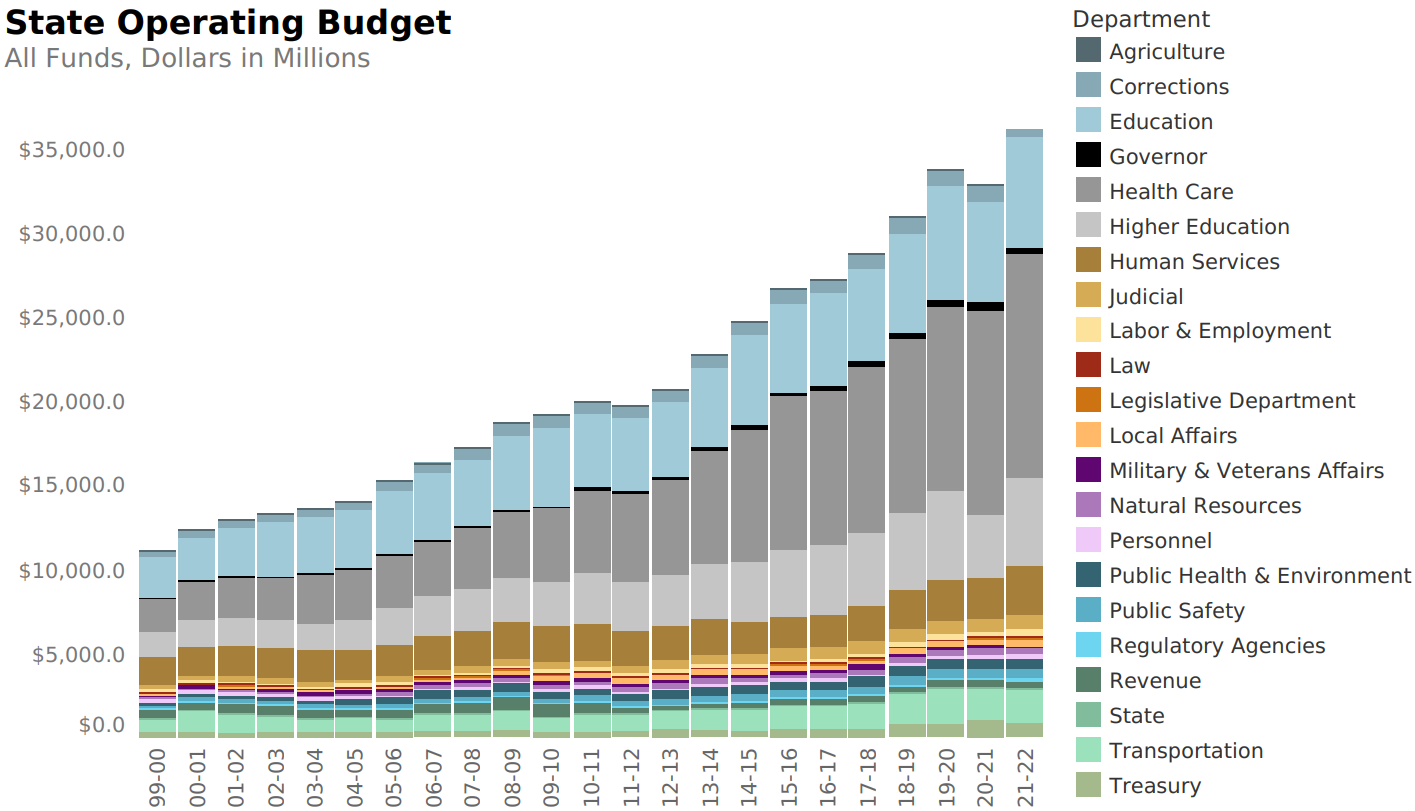
\includegraphics[width = 14	cm]{figures/Colorado_Budget.PNG}
	\caption{State of Colorado Budget}\label{fig:bud}
\end{figure}

Gieven that the contracts awarded through procurement auctions are such a substantial part of the budget, every potential improvement to the process in place may greatly increase the efficiency of the tax payers money spent. Accordingly, a closer examination of the process including a prediction model for the auctions' award prices may support public procurment agencies like the CDOT with budget planning. Additionally, further analysis of the underlying data in respect to the interactions of particular bidders and the associated effect on award prices is also highly relevant for public propcurement agencies. This thesis thus provides an analysis of different models, that predict the award price of an auction given input information available through the bid tabs that are published on the official website of the CDOT. In particular, four different model types with different preprocessing schedules are compared in terms of their predictive power. Standard linear regression, lasso regression, random forests and an eXtreme gradient boosting model. To assess, whether, the combination of certain bidders leads to higher award prices, recently discovered post-selection inference methods are utilized.\\
The remaining paper is strucutured as follows, first the data extraction process from the PDFs provided on the CDOT's website is described. Then the general process of procurement is described, once from the perspective of the auctioneer and also from the perspective of the competing firms. The following chapter then covers the methods used, not only in respect to the different models used for prediction but also for the different pre-procerssing shedules, that are applied and the post-selection inference that is used. The thesis then concludes with the results for the best predictive model utilizing linear and quadratic loss functions and the results of the analysis of bidder interactions.

\section{Data}\label{sec:data}

All the information about the procurement contracts, is obtainable through the bid tab archive on the official website of the Colorado Department of Transportation. The information is provided in PDF documents. In each of those documents the following information of the respective auction is provided.

\begin{itemize}
	\item A table listing all submitted bids, including a unique identifier for each of the participating bidders
	\item A contract description
	\item An engineer's estimate
	\item The contract ID
	\item The letting date
	\item Either the amount of time given to complete all the contractual obligations, or a completion due date
	\item The county in which the contract is to be completed in 
\end{itemize}

For illustrative purposes, Figure \ref{fig:bidtab} displays an example of a bid tab, in particular the second page, which contains the vendor ranking as well as the contract description and the remaining information listed above.

\begin{figure}[H]
	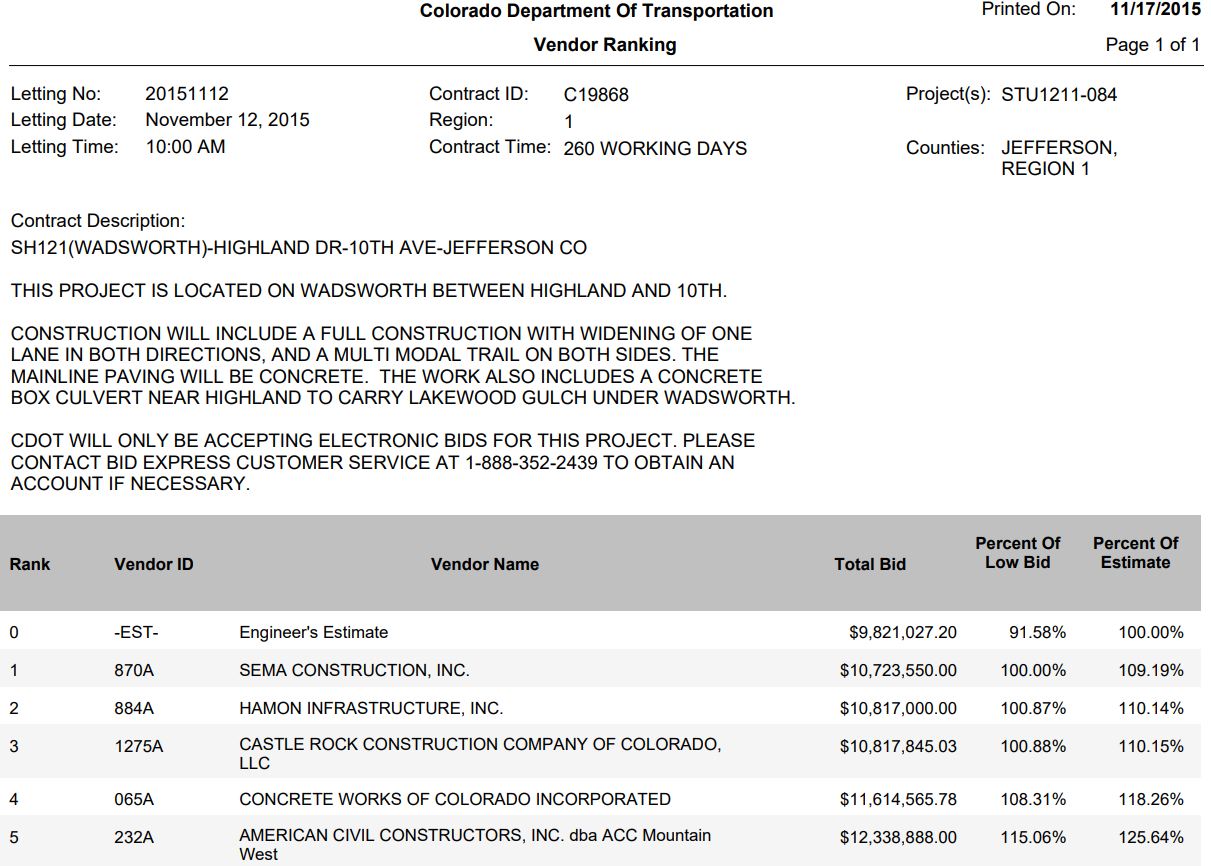
\includegraphics[width = 14	cm]{figures/Bid_Tab_exmpl.PNG}
	\caption{Bid Tab Example}\label{fig:bidtab}
\end{figure}

\subsection{Scraping}\label{subsec:scrap}
In order to obtain all the archived bid tabs, the html code of the website was first examined using a google chrome extension called SelectorGadget. This tool allows one to identify html nodes, that website contents are associated with. In the case of the bid tab archive, the html node carrying the links to the individual bid tabs is \enquote{<td a>}. Once this html node is discovered and the consistency across different years in the archive is ensured, the download is easily achieved by looping over the links and downloading the  respective PDFs. The hyperlink extraction was performed utilizing \textit{rvest}, by \citet{rvest}. For the remaining steps in the data extraction process, a distinction will be made for text based information and tabular data.

\subsubsection{Text Based Information}\label{subsubsec:descr}
 The structure of the text based information allows us to filter the individual parts via regular expressions. Especially, for the letting data, the contract ID, and the county this required no further data cleaning steps. Unfortunately, this is not the case for the contract time and the contract description.\\ 
 The contract time was not as straightforward to obtain, since the way it is reported is inconsistent across documents. Most of the time, it is reported as working days until all contractual obligations have to be fullfilled. Seldom, however, the bid tab contains a completion date instead. Accordingly, to achieve consistency across documents all completion dates were converted to contract time. This was achieved by first adding 60 days to the letting date, as this is the number of days that the Cdot reports as the expected time between the letting date and the start of the work on site. Then, the difference in days between the completion date and the starting date were computed. As, said difference is only supposed to contain working days the following holidays as well as all weekends were substracted from the difference betwen starting date and completion date.
 
 \begin{itemize}
 	\item New Year's Day
 	\item Dr. Martin Luther King, Jr. Day
 	\item President's Day
 	\item Memorial Day
 	\item Juneteenth
 	\item Independence Day
 	\item Labor Day
 	\item Frances Xavier Cabrini Day
 	\item Veterans Day
 	\item Thanksgiving
 	\item Christmas
 \end{itemize}
 
 The computation was executed utilizing the R package \textit{bizdays}, \citet{bizdays}. The package enables the user to generate custom calenders. The difference in starting and completion date was therefore easily calculated by setting up a custom calender with the holidays listed above as well as all saturdays and sundays. Then using this calender, the difference between two dates will only take working days into account.
 The only remaining text based information is the contract description. So far, none of the text based information required extensive preprocessing to obtain variables that can be represented in a tabular format. In the case of the contract description this is not the case. In order to convert the contract description into a format that may be represented in a table, the descriptions were first tokenized. Tokenization refers to splitting the input text into single unique words, i.e., splitting the sentences on spaces and removing all forms of punctuation. The result is then a vector of tokens. Said tokens were then scanned for spelling mistakes utilizing the R package \textit{hunspell} \citep{hunspell}. Once the misspelled words were corrected, stopwords were removed from the list of tokens. Stopwords are words that have no inherent signal associated with their use, examples for such words in the english language would be \enquote{a}, \enquote{is} and \enquote{the}. In natural language processing there is not necessarily one list of stopwords, depending on the context different libraries of stopwords may be used to remove as much noise as possible from textual data while leaving the signal associated with a series of words in tact. In the case of this thesis, a combination of five different libraries of stopwords was used. All of those libraries, \enquote{snowball} , \enquote{stopwords-iso}, 
 \enquote{smart}, \enquote{marimo} and \enquote{nltk} are available through the R package \textit{stopwords}, by \citet{stopwords}. After filtering out the stopwords, the remaining words were then stemmed. Stemming refers to the process in which a word is reduced to it's root. This means, that words that carry an identical signal are reduced to the same shortest common substring. Consider the following three words, replacing, replaced, replacement. All those words carry the information that something needs replacement. The language specific circumstances that determin the affixes are not relevant for the information extraction and thus all the aforementioned words are shortened to \enquote{replac} \citet{textminingR}. After stemming, to remove any remaining misspelled words and also for potential removal of unwanted information, all stemmed words were written to an excel file and checked manually. Given that all stopwords were already removed and the remaining words were reduced to their stem, this was a very feasible task, resulting in a file with around 2000 words to check. Below we observe the top 40 most frequent words that result from our text mining endeavours.
 
\begin{figure}[H]
	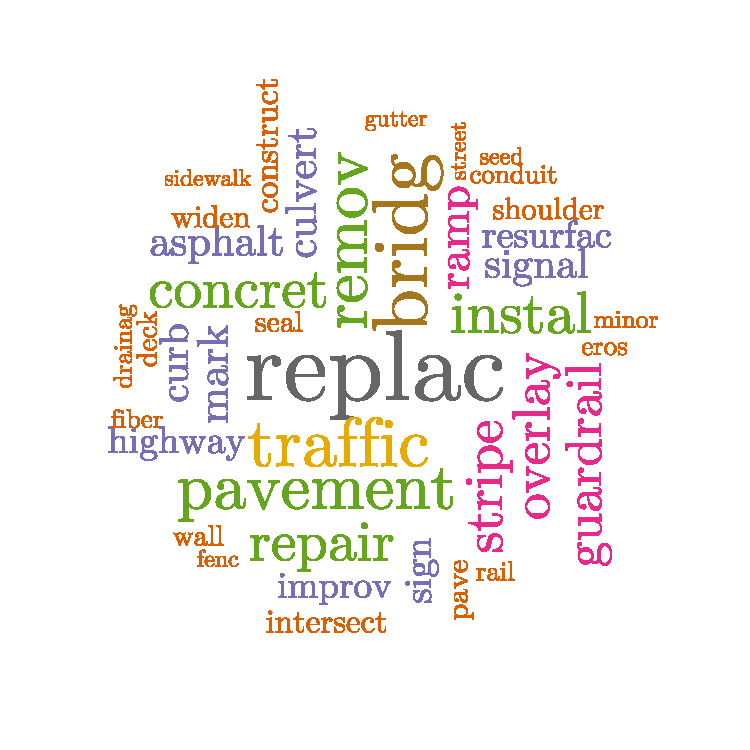
\includegraphics[width = 13.4	cm]{figures/description_words_cloud.pdf}
	\caption{Top 40 Stemmed Description Words}\label{fig:desc}
\end{figure}

\subsubsection{Tabular Data}\label{subsec:tab}

As displayed in Figure \ref{fig:bidtab}, the table in each of the auctions' PDFs contains information on the submited bids, the bidders' identity and an engineer's estimate. To extract the table containing this information, the package \textit{tabulizer} by \citet{tabulizer} is utilized. This package provides bindings for the Tabula PDF extractor, written in Java. In particular, two functions of the library were combined to write a wrapper for the table extraction. First the function \textit{extract\_tables()} was used to attempt automized table detection and subsequent extraction. Unfortunately, however, there are quite a few cases in which the automatic table detection failed because some auctions only have one or two bidders. The resulting tables that summarize those auctions have very few rows and thus the automatic detection does not recognize them as tables. Accordingly, if the output of \textit{extract\_tables()} is empty, the implemented wrapper calls \textit{extract\_areas()}. This function allows the user to specify an area via the R plot-pane to specify where exactly the table is located. Once the location is passed manually, which was necessary for around 10-15\% of cases, the extraction works as intended. To finally, obtain the tables the wrapper is used to loop over the PDFs.

\subsection{Descriptive Statistics}\label{subsec:desc}
The data that results from the sraping process is based on an auction level. Meaning that each of the 430 auctions that were scraped between 2015 and 2019 represents one row. The final columns are thus:

\begin{itemize}
	\item Contract ID
	\item County
	\item Letting month
	\item Letting year
	\item Contract time
	\item Number of bidders
	\item Engineer's estimate
	\item Award price
	\item 169 binary variables, representing the bidder identities
	\item 652 binary variables, representing pair-wise bidder interaction terms 
	\item 258 binary variables, representing the contract description hitwords
\end{itemize}

The interactionterms were generated in order to see, whether, a combination of certain bidders leads to a lower or higher award price. Those terms may also be used to perform unsupervised collusion detection utilizing post-selection inference for $\ell_1$-penalized models. This idea is further outlined in Section \ref{subsec:col}. To obtain a concise overview of the data,  histograms and barcharts of the variables are provided below.

\begin{figure}[H]
	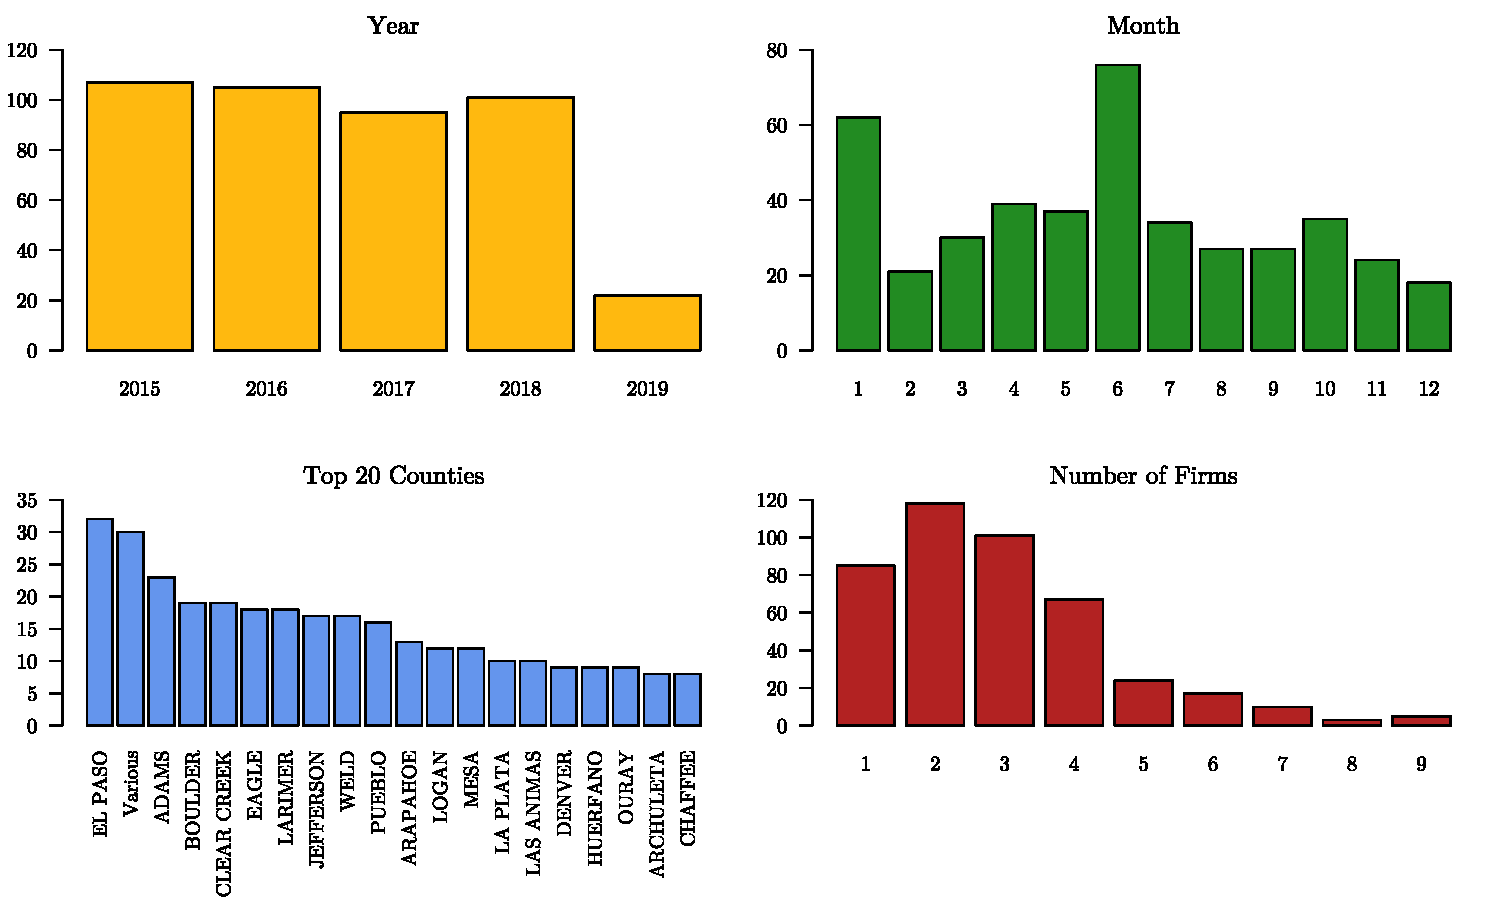
\includegraphics[width = 14	cm]{figures/barplots.pdf}
	\caption{Date, Counties and Number of Firms}\label{fig:barplots}
\end{figure}

We observe, that the sample of auctions in the dataset were held between 2015 and 2019, in which the auction frequency is the highest in January and June. Further we learn, that most contracts are to be completed in El Paso followed by a combination of multiple counties. In regards to the number of bidders per auction, most of the auctions have between 1 to 4 bidders, with the maximum being 9 competing firms.

\begin{figure}[H]
	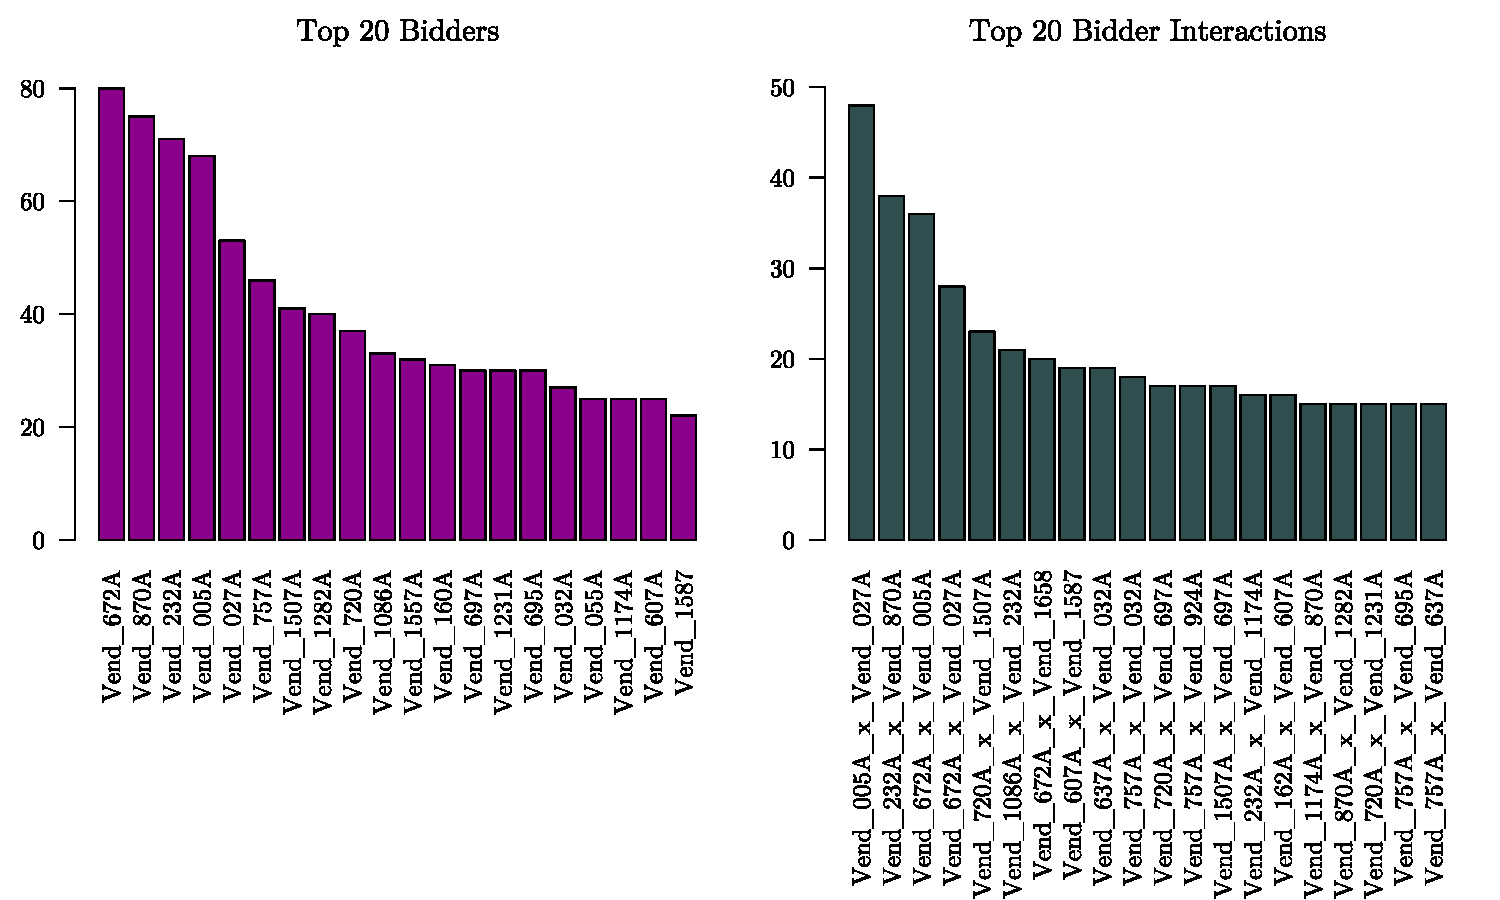
\includegraphics[width = 14	cm]{figures/vend_plots.pdf}
	\caption{Bidders and their Interactions}\label{fig:vendplots}
\end{figure}

The depiction of the top 20 bidders represents the unique identifiers of the firms that submitted the most bids. It is interesting to see that there seem to be a handful of firms that compete in drastrically more auctions than others. Additionally, we observe that the two firms that submitted the most bids in the same auctions, compete in slightly more than 10\% of the auctions in the dataset.

\begin{figure}[H]
	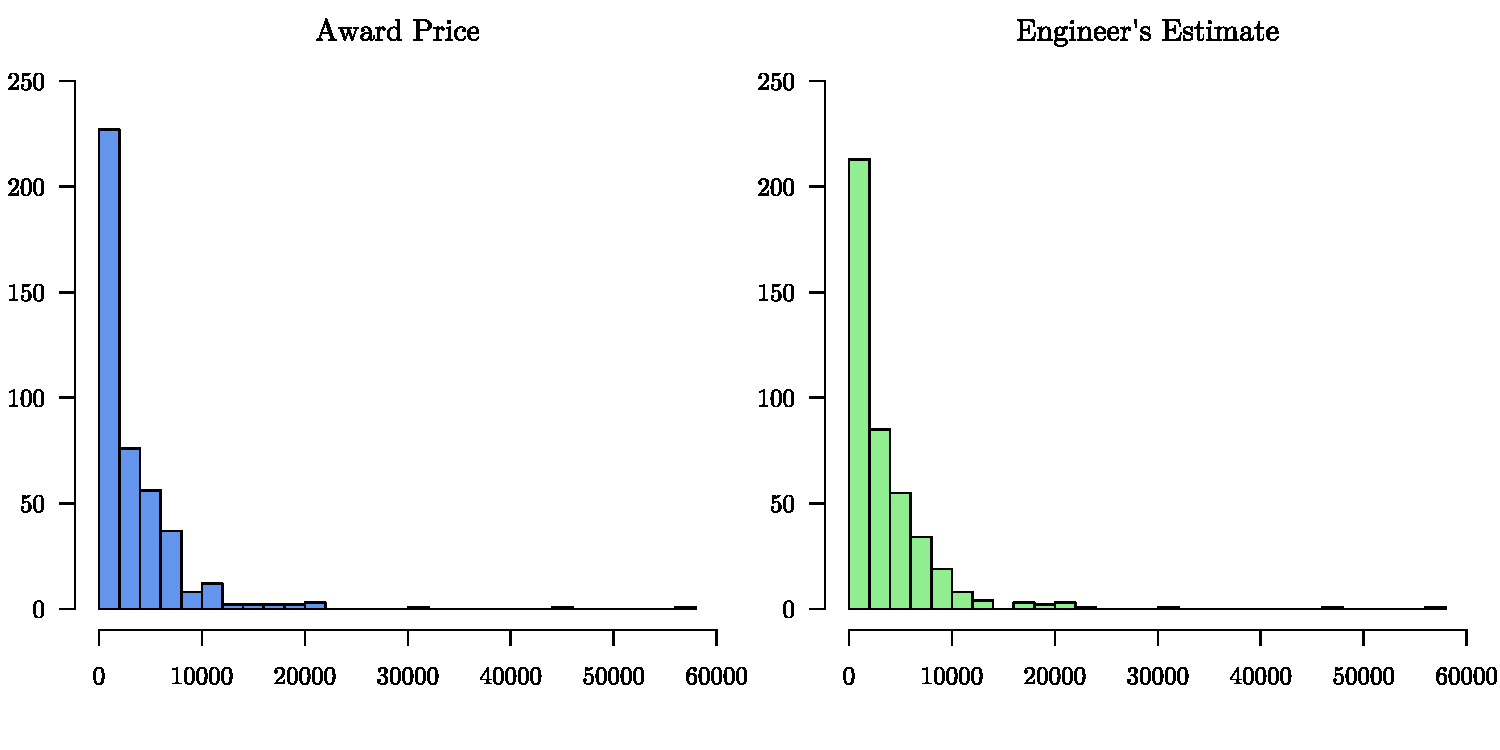
\includegraphics[width = 14	cm]{figures/aw_eng_hist.pdf}
	\caption{Award Price and Engineer's Estimate}\label{fig:aweng}
\end{figure}

The last two plots, enable us to gain insights about the distribution of the award price and the engineer's estimate. Both variables are right skewed and to the naked eye the engineer's estimate seems to resemble the distribution of the award price quite well. This is a strong indicator for the engineer's estimate as a predictor. The engineer's estimate is also important as it serves as a benchmark for prediction. Every model that can not beat the engineer's estimate in predicting the award price is not particularly useful, this is further discussed in Section \ref{sec:res}.\\

\section{Economic Operationalization}\label{sec:op}

Before formalization, a quick overview of the auction design of the Colorado Department of Transportation is presented. This renders modeling assumptions more comprehensible. The CDOT provides a document on their website that summarizes the entire auction process including all preregistration processes, that firms have to traverse before they are eligible to submit bids \citep{CDOTRul}.\\

The auction design created by the CDOT is a classical sealed-bid first-price auction, i.e., contracts are advertised for bids online, firms that have been prequalified for bidding for a certain contract may submit their bids online or in person. Once a preset date passes a representative of the CDOT opens all submitted bids and announces the lowest bidder, who is awarded the contract. The prequalification that was mentioned is of vital importance for this thesis. Given that all firms have to be prequalified for bidding, one may utilize bidder identity and bidder interactions when predicting award prices. If there was no prequalification, then the auctioneer would not have knowledge of all potential bidders until no more bids are to be received. At this point there is also no need of a prediction of the award price. Besides a prequalification process, the CDOT also implements a reserve price. Every project is assigned an engineer, who is responsible to calculate an engineer's estimate of the cost of completion. Should the lowest bid that was submitted exceed the engineer's estimate by more than 10\% then the lowest bidder is only awarded the contract if a secondary assessment of the CDOT ends with the conclusion that the lowest apparent bid is indeed a reasonable price for execution of the contractual obligations. This secondary process to bypass the initial reserve price was necessary for 17\% of the auctions in the dataset that is used in this thesis.

\subsection{First Price Sealed Bid Auctions}\label{subsec:fpsba}

For the applied nature of this thesis a formalization of the auction process in not a necesary prerequisite 
for a good prediction model, however, a sound understanding of all the economic agents at play might yield insights into the potential gains made from a prediction model for participating firms and may also provide us with expectations for the post-selection inference that is explored in Section \ref{subsubsec:psi}. Given that this chapter is not strictly necessary for the reader to understand the main findings of this thesis a basic understanding of game theory is assumed.\\
The description of bidding in the first-price sealed-bid procurement auction (FPSBPA) is denoted in accordance with \citet{milgrom82} and \citet{HandbookIndustrialOrga}. For the following description let uppercase letters represent random variables and their lowercase counterpart a single realisation. Consider an auction enviroment with $n$ potential bidding firms, all of them submit bids in hopes to procure a contract from the auctioneer. Each of those firms, which are indexed by $i$ observe a signal $x_i$. One can think of $X_i$ as private information that each firm has about their own cost structure. Further, let $V$ represent the characteristics that determin the value of the contract to the firms. Firm $i's$ payoff is represented by $U_i = u_i(V, X_i, X_{-i})$, where $X_{-i}$ represents the characterisitcs of firms $i's$ rivals. Most of the time it is assumed that firms are risk neutral, i.e., expected utility of profit is simply equal to the expectation of a linear function of capital gained, and maximizing it is equivalent to maximizing expected profit itself. Let the bidding strategy be a mapping $\beta: X_i \rightarrow \mathbb{R}^+$, that maps the characteristics of firm $i$ into the non-negative real numbers. To ensure that this function is invertible, in the literature it is usually assumed that $\beta$ is a bijection that is strictly increasing in the signals $X_i$, this is not particularly unrealistic. Again, assuming that $X_i$ represents the cost structure of firm $i$ a ceteris paribus decrease in costs is then associated with a decrease in the price of submitted bids. Now that the basic formalities of the auction enviroment have been set, we may consider the \enquote{winner's curse}, which assumes the event of winning an auction as an informative event in respect to the value of the contract. The idea is that a firm that manages to procure a contract through an auction must be the lowest bidder, and this also means that no other firm was willing to execute the contractual obligations for the same price. More formally, assume that the realization $v$ is unknown and identical for all firms, i.e, we are assuming that firms will be able to extract the same profit from this contract. Further, assume that the cost for completing of the contract is drawn from a common distribution $F$ and that the value of the contract to the firms is identical prior to the realisation of the cost draw, i.e, w.l.o.g for firm 1 the ex ante valuation of the contract is equal to:
\[
v_1(x_1) = \mathbb{E}[V|X_1 = x_1]  = \int vf_{V|X_1}(v|x_1)dv.
\]
 Then in equilibrium, assuming that the bidding function is increasing in the cost realization, the winner is the firm with the lowest cost draw from the distribution. By Jensens inequality, given that the maximum is a convex function, 
\[
\mathbb{E}[\text{max}\{V_i|v\}] \leq \text{max}\{{\mathbb{E}[V_i|v]}\} = v.
\] 
This represents the winner's curse as the firm with the lowest cost draw may extract the most profit. Further as \citet{milgrom82} state, w.l.o.g, for firm 1 this means:
\[
\mathbb{E}[V|X_1 = x, Y_1 > x] < \mathbb{E}[V, X_1 = x].
\]
Where $Y_1$ is the firm with the lowest cost of contract execution among firm 1's rivals. We thus find that the bidder that incurs the lowest cost associated with the completion of all contractual obligations and therefore the highest potential profit to be extracted from the procurment of the contract should bid less than the firm's ex ante estimate of $V_1$, simply because the assignment of the contract to the firm as the lowest bidder is an informative event. Especially for firms, that are not as established and might have difficulties to obtain the expertise to properly assess the difficulties associated with completion of a contractual agreement will suffer more severly from the winner's curse. This is relevant for this thesis as an award price prediction that gives a reasonable estimate for the costs associated with the completion of a contract will change the informational assymetries and thus also lessen the severity of the winner's curse, should the award price prediction be shared with the bidders \citep{GarciaRodriguez2020}.\\

Now that we have discovered another potential beneficiary of a award price prediction model, we may assess the strategic bidding behaviour of firms. To further simplify the strategic behaviour we may again assume that firms cost realisations $x_i$ are drawn from a common distribution $F$, further we may asssume that the number of firms that submit bids is common knowledge and that the reserve price is not binding. Essentially, that means that the firms believe that bidding above the 110\% treshhold will not lead to a reissue of the contract but to a contract award in the secondary process previously described.
Given that this game is symmetric, we may again focus on firm 1 w.l.o.g. The firm aims to maximize its expected profit, i.e.,
\[
\argmaxA_b \text{ } (b - x)\{1 - F[\beta^{-1}(b)]\}^{n-1},
\]
which is just the expected profit. Where $(b - c)$ is the profit that the firm expects if it were to win the contract and the remaining term is the probability that all other competing firms have higher costs associated with the execution of the contractual obligation, and thus submit higher bids. Accordingly, by the previously mentioned assumption of the strictly increasing function $\beta$, the lowest cost realization leads to the lowest bid. From the maximization problem, we obtain the following FOC:
\begin{gather*}
	\{1-F[\beta^{-1}(b)]\}^{n-1} + (b - x)(n - 		1)\{1-F[\beta^{-1}(b)]\}^{n-2}\frac{d\beta^{-1}}{db}\{(-1)f[\beta^{-1}(b)]\} \overset{!}{=} 0\\
	\frac{\{1-F[\beta^{-1}(b)]\}^{n-1}}{\{1-F[\beta^{-1}(b)]\}^{n-2}} = (b - x)(n - 1)f[\beta^{-1}(b)]\frac{d\beta^{-1}}{db}\\
	1-F[\beta^{-1}(b)] = (b - x)(n - 1)f[\beta^{-1}(b)]\frac{d\beta^{-1}}{db}
\end{gather*}
Knowing that in the bayesian NE, $\beta^{-1}(b) = x$ and $\frac{d\beta^{-1}(b)}{db} = \frac{1}{\beta'(x)}$, we then find:
\begin{gather*}
	\beta'(x) = \frac{[\beta(x) - x](n - 1)f(x)}{1-F(x)}
\end{gather*}
This is a differential equation that modern computer algebra systems like mathematica can easily solve to obtain the bayesian NE bid function.
\[
\beta(x) = x + \frac{\int_x^\infty [1 - F(t)]^{(n-1)}dt}{[1-F(x)]^{(n-1)}}
\]
We thus learn that the bid resulting from the cost structure of the firm is a surcharge added to the cost realization. Further, we observe that the surcharge depends on the number of firms in an auction and the common cost distribution. We have to keep in mind, however, that this simple result is based on quite restrictive assumptions. Especially, the risk neutrality of firms is not particularly realistic and it is also not very plausible that all cost realizations are drawn from the same distribution. This would imply that economies of scale do not play a role. Nonetheless, given those simplifying assumptions, the results displayed in section \ref{sec:res} will show whether the derived economic intuition of firms behaviour is observable in the data.
\section{Methods}\label{sec:meth}

This section contains precise descriptions of the methods used to generate the results presented in section \ref{sec:res}.

\subsection{Elastic Nets}\label{subsec:net}

When the amount of features in a dataset is significantly larger than the amount of observations, elastic net regularization offers a solution to fit linear models using a convex combination of the lasso and ridge penalty.\\
The description of the elastic net regularization is denoted in accordance with the seminal paper by \citet{hastie03}. Assume that a dataset has n observations and p explanatory variables. As it is the case with the award price datset, the number of explanatory variables may greatly exceed the number of observations, i.e., $p >> n$. Let $\mathbf{y} = (y_1, ...., y_n)^T$ be the response variable and $\mathbf{X} = [x_1|...|x_p]$ the model matrix, containing the hot encoded explanatory variables. This means that all factor variables have to be converted to individual dummy variables for each level. Subsequently, each column in the model matrix is then centered and standardized. This ensures that the regularization is consistent across variables, since the regularization process is not scale invariant. For any combination of non-negative $\lambda_1$ and $\lambda_2$, \citet{hastie03}, define the elastiv net criterion as,
\[
L(\lambda_1, \lambda_2, \bm{\beta}) = |\mathbf{y} - \mathbf{X}\bm{\beta}|^2 +\lambda_2|\bm{\beta}|^2 +\lambda_2|\bm{\beta}|_1, 
\]
where $|\bm{\beta}|^2$ represents the $\ell_2$ norm of the coefficient vector $\bm{\beta}$, i.e., 
\[
|\bm{\beta}|^2 = \mathlarger{\sum}\limits_{i = 1}^{p}\bm{\beta}_i^2
\]
and $|\bm{\beta}|_1$ is equivalent to the $\ell_1$ norm, i.e.,  
\[
|\bm{\beta}|_1 = \mathlarger{\sum}\limits_{i = 1}^{p}|\bm{\beta}|.
\]
The elastic net estimator $\bm{\hat{\beta}}$ results from the following minimization problem,
\[
\bm{\hat{\beta}} = \argminA_{\bm{\beta}} L(\lambda_1, \lambda_2, \bm{\beta}).
\]
Alternatively, the elastic net penalized regression may also be written as a constrained optimization problem of the least square estmator. Let $\alpha = \frac{\lambda_2}{\lambda_2 + \lambda_1}$, then for some fixed $t$, 
\[
\bm{\hat{\beta}} = \argmaxA_{\bm{\beta}} |\mathbf{y} - \mathbf{X}\bm{\beta}|^2,
\]
subject to,
\[
(1 - \alpha)|\bm{\beta}|_1 + \alpha|\bm{\beta}|^2 \leq t.
\]
The constraint thus encompasses a convex combination of the lasso penalty and the ridge penalty. Accordingly, both ridge and lasso regression are a special cases of an elastic net, where $\alpha = 1$ results in ridge regression and $\alpha = 0$ leaves us with the $\ell_1$ penalized lasso regression estimator.

\subsubsection{Post-Selection Inference for $\ell_1$-Penalized Models}\label{subsubsec:psi}
\subsection{Ensemble Methods}\label{subsec:ens}
\subsubsection{Random Forests}\label{subsubsec:rf}
\subsubsection{eXtreme Gradient Boosting}\label{subsubsec:xgb}
\subsection{Nested Cross Validation}\label{subsec:nest}
\subsubsection{Logistic PCA}\label{subsubsec:logp}
\subsubsection{Recursive Feature Elimination}\label{subsubsec:rfe}
\section{Results}\label{sec:res}
\subsection{Prediction}\label{subsec:pred}
\subsubsection{Performance Evaluation Metrics}\label{subsubsec:per}
\subsection{Unsupervised Colusion Detection}\label{subsec:col}
\section{Conclusion}\label{sec:con}
 
\newpage
\printbibliography
\end{document}